\chapter{DATA ANALYSIS}\label{ch3}

The first section of this chapter includes an overview of the simulation of the proton-proton collisions and the second part explains the details of the prospects for nonresonant Higgs boson pair production measurements at the HL-LHC in pp collisions with a centre-of-mass energy of $\sqrt{s}=14\;TeV$

\section{Simulation and Reconstruction of Proton-Proton Collisions}

Simulation of a pp collision starts by describing the hard interactions which is done by Monte Carlo (MC) simulations. A number of different methods are used in these simulations in order to model the matrix element, consequently the cross section of the process of interest. 

\subsection{Event Generation}

The event generation is the first step of the simulation of the high energy collisions. The Monte Carlo techniques are used to simulate the events which happen in the actual collider experiments. The collisions between the protons at the LHC, takes place infact between the constituents of the protons, called partons to denote the quark and gluon content. In the pp collisions, not only two partons from different protons collide, which produces an interesting event to study, but also two partons can interact but not hardly. The different types of interactions that may occur in the collisions are shown in \autoref{eventtypes}. The \emph{\bf{hard scattering}} processes occur by the high exchange of momentum between the consitituents of two colliding protons. The products of this type of interaction usually have high transverse momenta. The high energetic partons may also emit radiation in the initial and final states, creating parton showers which is a considerable effect and taken into account in the event generation process.

\begin{figure}[ht]
	\centering
	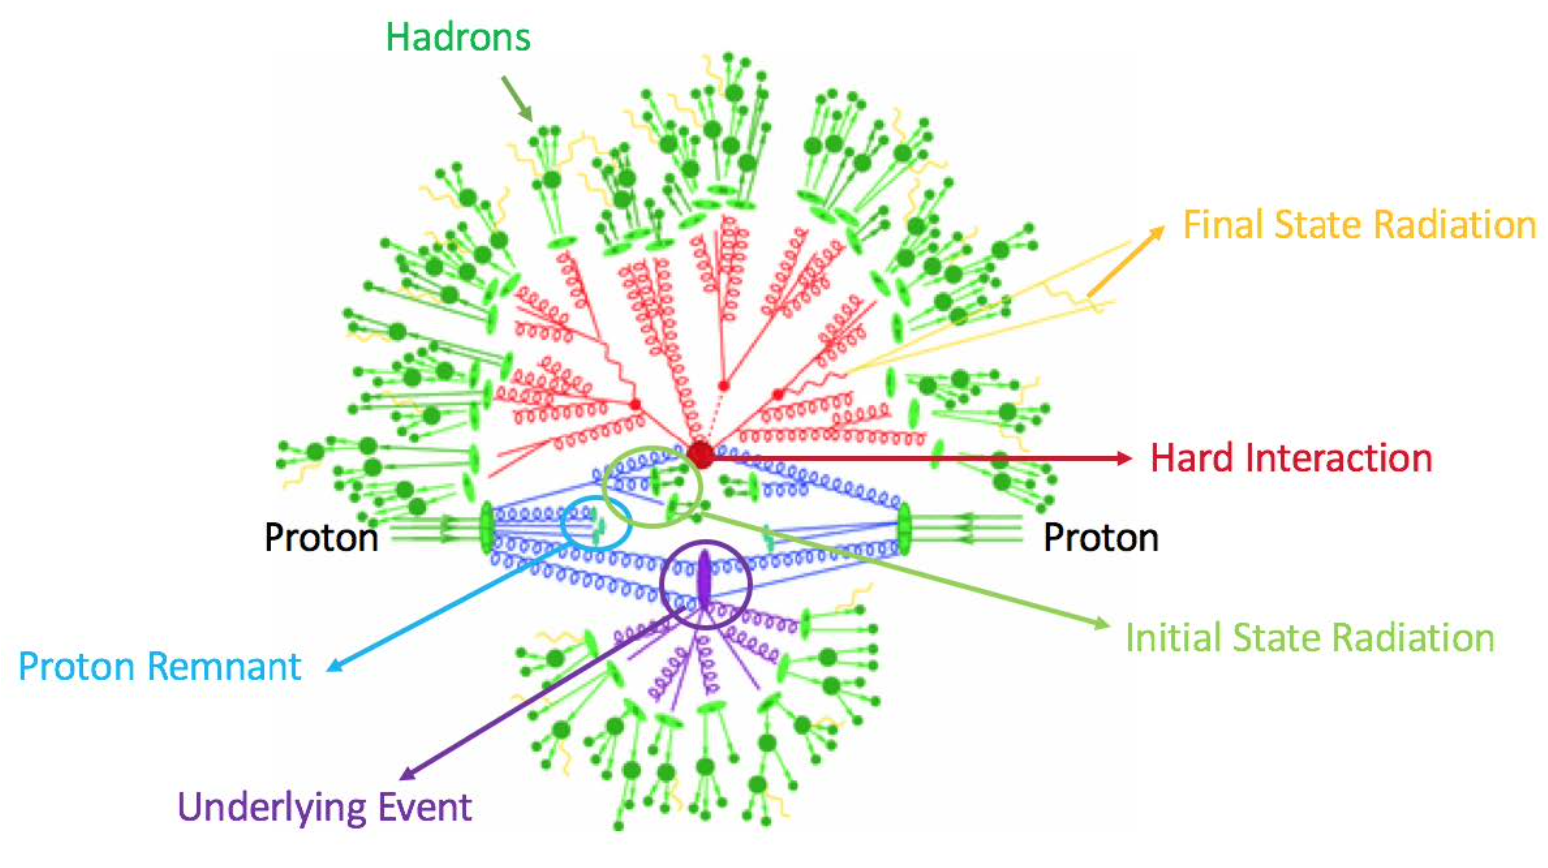
\includegraphics[width=\textwidth]{eventtypes.png}
	\vspace{2mm}
	\caption[Graphical representation of a pp collision event. The proton beams come from the either sides. The red diagram shows the hard interaction and the consequent decay of the products. A secondary interaction before the final state partons hadronise, is shown in purple. The hadronisation is indicated in green.]
	{Graphical representation of a pp collision event. The proton beams come from the either sides. The red diagram shows the hard interaction and the consequent decay of the products. A secondary interaction before the final state partons hadronise, is shown in purple. The hadronisation is indicated in green \cite{Pttgen2016}.}
	\label{eventtypes}
\end{figure}

An \emph{\bf{underlying event}} is soft interaction that occurs between the residue of the protons which have not taken place in the hard interaction. The partons may also radiate gauge bosons before or after interacting with each other, called initial state radiation and final state radiation, respectively. Additionally, partons can emit radiation via the strong interactions which create jets close to the direction of the initial particles.

At the LHC, bunches including $10^{11}$ protons are collided and pile-up processes, any type of interactions outside the hard scatterings, constitute a significant effect in the event generation. Another aspect of the pp collisions that needs to be considered in MC simulations is the hadronisation process. It is the merger process of quarks and gluons to form colourless, and seen in the final states. The hadronisation process occurs if the partons reach the energy scale of about 1 GeV. The creation of a colourless primary hadrons from partons is decribed in two different models; the \emph{\bf{cluster model}} and \emph{\bf{the string model}}. The former decribes the forming of the colourless hadrons by the gluons that are split into quark-antiquark pairs which then combines as colourless groups. The states clustered in this manner usually possess a large invariant mass which consequently decay to lower mass states convenient to create hadrons \cite{Webber1984}. In the latter model, the gluons are thought to be split into quark pairs that move away from each other where a string-like configuration is formed between them. As the string is stretched, its potential energy increases lowering the kinetic energy. The string eventually breaks in two creating a quark-antiquark pair. The mechanism is repeated until there is no energy left for another quark pair to be created \cite{Andersson1983}.

Various theoretical, phenomenological and experimental inputs are injected in to MC simulations in order to produce a consistent description of the pp collisions. Different approaches are utilised, for example in order to describe the QCD induced processes which have varying phenomenology with the changing energy scale \cite{skands2012qcd}. The hadronic cross section $\sigma_{pp}$ is calculated using the QCD factorisation theorem, which decribing it as a convolution integral of the partonic cross section $\hat\sigma_{ij}$ with the parton distribution functions $f_i(x)$:

\be
\sigma_{pp} = \int_{x_{min}}^1 f_i(x_1)f_j(x_2)\hat\sigma_{ij}(x_1p_1, x_2p_2)dx_1dx_2 \; ,
\ee

where $f_i(x)$ in the probability density that a parton of type $i$ has a fraction x of the hadron's energy.

The overall chain of calculating a process includes; i) the PDF, which is basically the phenomenological interpretations calculated with the information coming from the experiments, ii) the hard scattering, calculated in perturbatively in orders, iii) the parton shower process, the radiations in perturbative QCD, iv) the hadronisation, lays out the forming of colourless hadrons from coloured partons based on phenomenological models, and v) the decay of unstable particles treated using experimental data. The first two steps are usually calculated in Matrix Elements generators, while the rest is usually calculated in parton shower software. MC techniques are used in both sides and the transition is made in a manner to avoid double counting of the QCD radiation.

\subsection{Detector Simulation}

\subsection{Reconstruction of Physics Objects}

\section{Analysis}

\subsection{Signal and Background Samples}

In this thesis, signal ($gg \rightarrow HH$) samples are generated using Powheg v2 \cite{Nason2004, Frixione2007, Alioli2010, Heinrich2019} at next-to-leading order (NLO) in QCD including the full top mass dependence with SM parameters, and subsequent decays of the Higgs boson pairs into $\tau\tau$, $WW$ and $ZZ$ each with a photon pair is implemented using PYTHIA 8.212 \cite{Sjstrand2015}. The signal samples for three seperate final states of \wwgg channel are produced while a single sample including all possible decays of taus are used.

The analysis is overwhelmed by non-resonant backgrounds with continuum \mgg spectra and by single Higgs boson productions. The sample generation for single Higgs productions is performed via MadGraph5\_aMCatNLO \cite{Alwall2014, Artoisenet2013} with the FxFx merging scheme \cite{Frederix2012} for the gluon fusion (ggFH), vector boson fusion (VBFH), associated production with a vector boson (VH) and associated production with a top quark pair (ttH), while the top quark associated production  with a Higgs boson (tHq) was perfomed using MadGraph version-2.7 at LO.

Several SM processes contribute to the continuum background. A large portion of the dominant backgrounds across all final states comes from the $\gamma\gamma+$jets processes that are modelled with SHERPA v.2.2.1 generator \cite{10.21468/SciPostPhys.7.3.034}while QCD-induced processes, $\gamma+$jets and WW processes are modelled with PYTHIA 8 generator. W production in association with photons and jets, and Drell-Yan processes are modelled with MadGraph5 version-2.7 at LO, $t\bar t$ with Powheg v2, and $t\bar tW$, $t\bar t\gamma$, $t\bar t\gamma\gamma$, $Z\gamma$ processes with Madgraph5\_aMCatNLO.

\subsection{Object Selection}

\subsection{Event Selection and Categorisation}

\subsection{Bamboo Framework}

\subsection{Deep Neural Network Employment}

\subsection{Systematic Uncertainties}

\section{Results}